\documentclass[a4paper,12pt]{book}
\usepackage[utf8]{inputenc}
\title{}
\author{Rachel Morris}
\date{\today}

\usepackage{rachwidgets}
\usepackage{fancyhdr}
\usepackage{lastpage}
\usepackage{dirtree}
\usepackage{boxedminipage}

\newcommand{\laClass}{CS 211\ }
\newcommand{\laSemester}{Fall 2017\ }
\newcommand{\laChName}{Graphs in Puzzles and Games\ }
\newcounter{question}

\setcounter{chapter}{7}
\setcounter{section}{4}
\newcommand{\laChapter}{7.5 \laChName}

\pagestyle{fancy}
\fancyhf{}
\lhead{\laClass Exercise, \laSemester}
\chead{}
\rhead{Ch \laChapter}
\rfoot{\thepage\ of \pageref{LastPage}}
\lfoot{\scriptsize Compiled by Rachel Morris, last updated \today}

\renewcommand{\headrulewidth}{2pt}
\renewcommand{\footrulewidth}{1pt}

\begin{document}

    %\toggletrue{answerkey}
    \togglefalse{answerkey}

    \section{\laChName}
    
    \notonkey{

    %- Team Info ------------------------------------------------------%

    Please write down all people in your team. ~\\

    % table %
    \begin{tabular}{ p{6cm} p{6cm} }
        1. & 2. \\ \\
        3. & 4.
    \end{tabular} ~\\
    % table %
    
    \hrulefill
    
    }{}


    \subsection{Wolves, Goats, and Cabbages}

    \notonkey{
        \begin{introNOHEAD}{}
            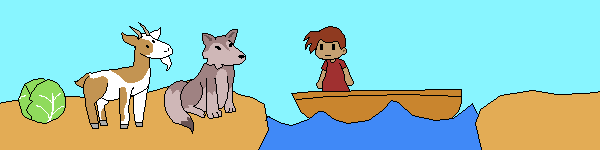
\includegraphics[width=13cm]{images/7-5-goats.png}
            
            A traveler has three possessions: a wolf, a goat, and a cabbage.
            They must transport them across a river.

            ~\\
            The catch is that,
            if left alone, the wolf will eat the goat, or the goat
            will eat the cabbage. The boat can only hold the traveller
            and one possession at a time.
            \footnote{Discrete Mathematics, Ensley and Crawley}

            ~\\
            For this problem, we are concerned with what valid states are.
            We can draw a diagram to represent all possible moves between
            the starting point (everything at the starting location)
            and the ending point (everything at the ending location) to
            help us solve it.

            Let's use $(WC,TG)$ to mean that the Wolf and Cabbage are
            left on the departing shore, and the Traveller and the Goat
            are on the arriving shore. If we write $(WCTG, \emptyset)$,
            then all four are on the departing shore, and nothing is
            on the arriving shore.

            \begin{center}
                \scriptsize 
                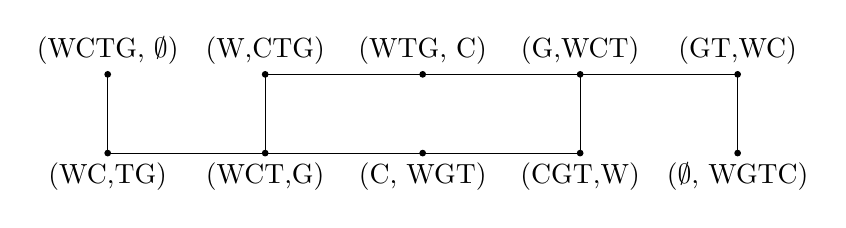
\begin{tikzpicture}
                    \filldraw (0,0) circle (1pt) node [below] {(C, WGT)};
                    \filldraw (0,1) circle (1pt) node [above] {(WTG, C)};
                    
                    \filldraw (-2,0) circle (1pt) node [below] {(WCT,G)};
                    \filldraw (-2,1) circle (1pt) node [above] {(W,CTG)};
                    
                    \filldraw (2,0) circle (1pt) node [below] {(CGT,W)};
                    \filldraw (2,1) circle (1pt) node [above] {(G,WCT)};
                    
                    \filldraw (-4,0) circle (1pt) node [below] {(WC,TG)};
                    \filldraw (-4,1) circle (1pt) node [above] {(WCTG, $\emptyset$)};
                    
                    \filldraw (4,0) circle (1pt) node [below] {($\emptyset$, WGTC)};
                    \filldraw (4,1) circle (1pt) node [above] {(GT,WC)};

                    \draw (-4,1) -- (-4,0) -- (-2,0) -- (0,0) -- (2,0) -- (2,1);
                    \draw (4,0) -- (4,1) -- (2,1) -- (0,1) -- (-2,1) -- (-2,0);
                \end{tikzpicture}
            \end{center}
        \end{introNOHEAD}
    }{}

\notonkey{ \newpage }{ \hrulefill }

% -------------------------------------------------------------%
% - QUESTION --------------------------------------------------%
% -------------------------------------------------------------%
\stepcounter{question}
\begin{question}{\thequestion}{8}

    Write a path (a list of vertices), starting at $(WCTG, \emptyset)$ and ending at $(\emptyset, WGTC)$,
    traversing the graph of valid states given.
    
        \begin{center}
            \footnotesize
            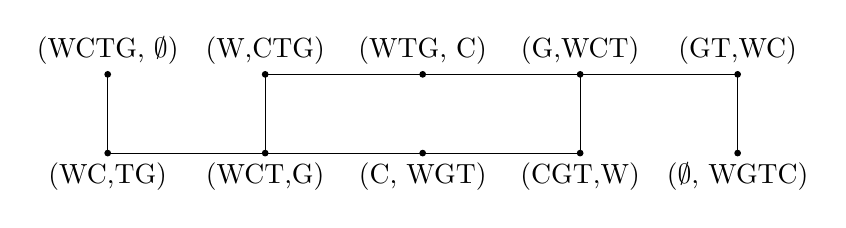
\begin{tikzpicture}
                \filldraw (0,0) circle (1pt) node [below] {(C, WGT)};
                \filldraw (0,1) circle (1pt) node [above] {(WTG, C)};
                
                \filldraw (-2,0) circle (1pt) node [below] {(WCT,G)};
                \filldraw (-2,1) circle (1pt) node [above] {(W,CTG)};
                
                \filldraw (2,0) circle (1pt) node [below] {(CGT,W)};
                \filldraw (2,1) circle (1pt) node [above] {(G,WCT)};
                
                \filldraw (-4,0) circle (1pt) node [below] {(WC,TG)};
                \filldraw (-4,1) circle (1pt) node [above] {(WCTG, $\emptyset$)};
                
                \filldraw (4,0) circle (1pt) node [below] {($\emptyset$, WGTC)};
                \filldraw (4,1) circle (1pt) node [above] {(GT,WC)};

                \draw (-4,1) -- (-4,0) -- (-2,0) -- (0,0) -- (2,0) -- (2,1);
                \draw (4,0) -- (4,1) -- (2,1) -- (0,1) -- (-2,1) -- (-2,0);
            \end{tikzpicture}
        \end{center}

        \begin{itemize}
            \item[a.]   Path:
                \solution{
                    (WCTG, $\emptyset$) - (WG, TG) - (WCT, G) - (C, WGT) - (CGT, W) - (G, WCT) - (GT, WC) - ($\emptyset$, WGTC)
                }{ \vspace{3cm} }
                
            \item[b.]   In $(WC, TG)$, what does the item to the left of the comma represent?
                \solution{
                    The characters on the ``beginning'' island.
                }{ \vspace{1cm} }
                
            \item[c.]   In $(WC, TG)$, what does the item to the right of the comma represent?
                \solution{
                    The characters on the ``destination'' island.
                }{ \vspace{1cm} }
                
            \item[d.]   What does $W$ represent?
                \solution{
                    The Wolf's position
                }{ \vspace{0.5cm} }
                
            \item[e.]   What does $C$ represent?
                \solution{
                    The Cabbage's position
                }{ \vspace{0.5cm} }
                
            \item[f.]   What does $T$ represent?
                \solution{
                    The Traveller's position
                }{ \vspace{0.5cm} }
                
            \item[g.]   What does $G$ represent?
                \solution{
                    The Goat's position
                }{ \vspace{0.5cm} }
                
            \item[h.]   What does $\emptyset$ represent?
                \solution{
                    That there are no characters at that position
                }{ \vspace{0.5cm} }
                
        \end{itemize}

    
\end{question}

\newpage


% -------------------------------------------------------------%
% - QUESTION --------------------------------------------------%
% -------------------------------------------------------------%
\stepcounter{question}
\begin{question}{\thequestion}{5}
    
    Given a tic-tac-toe board with the given starting state,
    draw a state diagram for all following valid moves until
    a win. Assume that it is X's turn next.
    \footnote{Diagram from http://neverstopbuilding.com/minimax}

    \begin{center}
        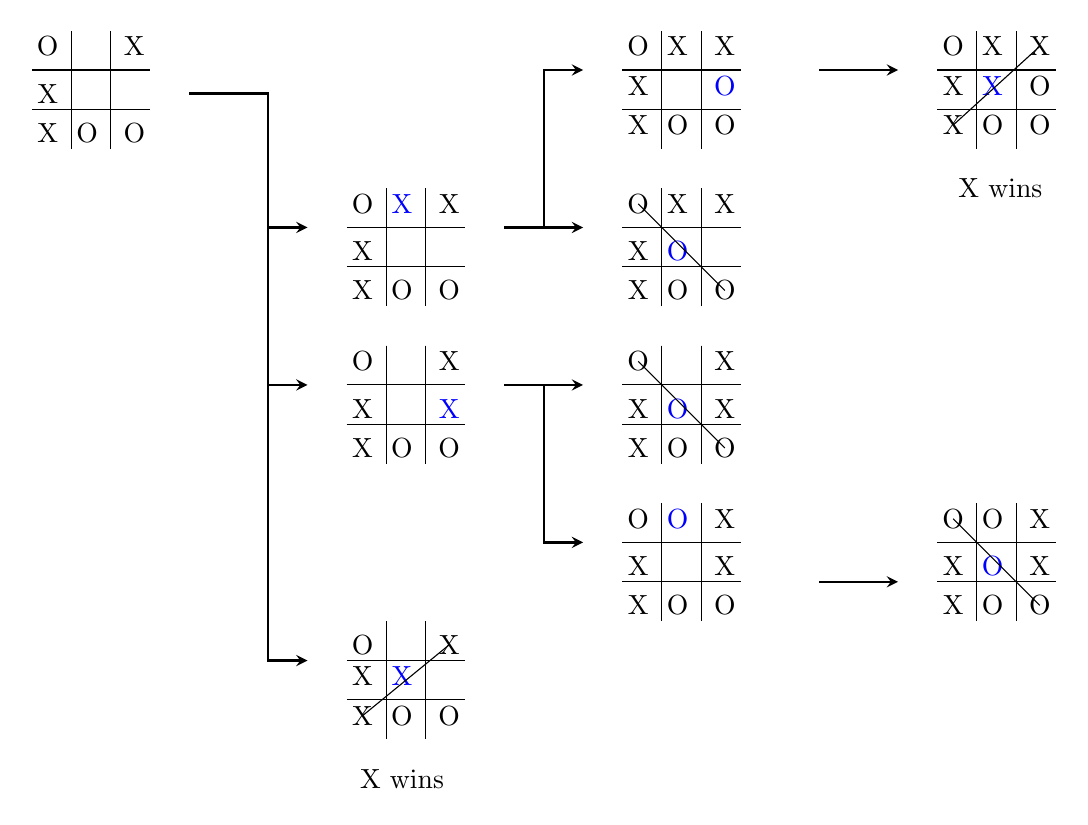
\begin{tikzpicture}[arrow/.style = {thick,-stealth}]

            \draw (0.5,1)   -- (0.5,2.5);
            \draw (1,1)     -- (1,2.5);
            \draw (0,1.5)   -- (1.5,1.5);
            \draw (0,2)     -- (1.5,2);
            
            \node at (0.2,2.3) {O};
            \node at (1.3,2.3) {X};
            \node at (0.2,1.7) {X};
            \node at (0.2,1.2) {X};
            \node at (0.7,1.2) {O};
            \node at (1.3,1.2) {O};

            \draw[arrow] (2,1.7) -- (3.0,1.7) -- (3.0, -5.5) -- (3.5, -5.5);

                % 2nd column, 5th row diagram
                \draw           (4.5,   -5)      -- (4.5,    -6.5);
                \draw           (5,     -5)      -- (5.0,    -6.5);
                \draw           (4,     -5.5)    -- (5.5,    -5.5);
                \draw           (4,     -6)      -- (5.5,    -6);
                
                \node at        (4.2,   -5.3) {O};
                \node at        (5.3,   -5.3) {X};
                \node[blue] at  (4.7,   -5.7) {X};
                \node at        (4.2,   -5.7) {X};
                \node at        (4.2,   -6.2) {X};
                \node at        (4.7,   -6.2) {O};
                \node at        (5.3,   -6.2) {O};

                \draw (4.2, -6.2) -- (5.3, -5.3);

                \node at (4.7, -7) {X wins};

            \draw[arrow] (3,0) -- (3.5,0);

                % 2nd column, 2nd row diagram
                \draw           (4.5,   0.5)    -- (4.5,    -1);
                \draw           (5,     0.5)    -- (5.0,    -1);
                \draw           (4,     -0.5)   -- (5.5,   -0.5);
                \draw           (4,     0)      -- (5.5,    0);
                
                \node at        (4.2,   0.3) {O};
                \node at        (5.3,   0.3) {X};
                \node[blue] at  (4.7,   0.3) {X};
                \node at        (4.2,   -0.3) {X};
                \node at        (4.2,   -0.8) {X};
                \node at        (4.7,   -0.8) {O};
                \node at        (5.3,   -0.8) {O};

            \draw[arrow] (6,-0) -- (6.5,-0) -- (6.5, 2) -- (7, 2);
            \draw[arrow] (6.5,-0) -- (6.5, -0) -- (7,-0);

            \draw[arrow] (3,-2) -- (3.5,-2);

            % 2nd column, 3rd row diagram
            \solution{
                \draw           (4.5,   -1.5)       -- (4.5,    -3);
                \draw           (5,     -1.5)       -- (5.0,    -3);
                \draw           (4,     -2)         -- (5.5,    -2);
                \draw           (4,     -2.5)       -- (5.5,    -2.5);
                
                \node at        (4.2,   -1.7) {O};
                \node at        (5.3,   -1.7) {X};
                \node[blue] at  (5.3,   -2.3) {X};
                \node at        (4.2,   -2.3) {X};
                \node at        (4.2,   -2.8) {X};
                \node at        (4.7,   -2.8) {O};
                \node at        (5.3,   -2.8) {O};
            }{
                \draw           (4.5,   -1.5)       -- (4.5,    -3);
                \draw           (5,     -1.5)       -- (5.0,    -3);
                \draw           (4,     -2)         -- (5.5,    -2);
                \draw           (4,     -2.5)       -- (5.5,    -2.5);
            }

            \draw[arrow] (6,-2) -- (7,-2);
            \draw[arrow] (6.5,-2) -- (6.5, -4) -- (7,-4);
                
            \solution{
                \draw           (8.0,     -1.5)     -- (8.0,    -3);
                \draw           (8.5,     -1.5)     -- (8.5,    -3);
                \draw           (7.5,     -2)       -- (9,      -2);
                \draw           (7.5,     -2.5)     -- (9,      -2.5);
                
                \node at        (7.7,   -1.7) {O};
                \node at        (8.8,   -1.7) {X};
                \node at        (8.8,   -2.3) {X};
                \node at        (7.7,   -2.3) {X};
                \node at        (7.7,   -2.8) {X};
                \node at        (8.2,   -2.8) {O};
                \node at        (8.8,   -2.8) {O};
                \node[blue] at  (8.2,   -2.3) {O};

                \draw (7.7, -1.7) -- (8.8, -2.8);
            }{
                \draw           (8.0,   -1.5)       -- (8.0,    -3);
                \draw           (8.5,     -1.5)     -- (8.5,    -3);
                \draw           (7.5,     -2)       -- (9,      -2);
                \draw           (7.5,     -2.5)     -- (9,      -2.5);
            }

            \solution{
                \draw           (8.0,     -3.5)     -- (8.0,    -5);
                \draw           (8.5,     -3.5)     -- (8.5,    -5);
                \draw           (7.5,     -4)       -- (9,      -4);
                \draw           (7.5,     -4.5)     -- (9,      -4.5);
                
                \node at        (7.7,   -3.7) {O};
                \node at        (8.8,   -3.7) {X};
                \node at        (8.8,   -4.3) {X};
                \node at        (7.7,   -4.3) {X};
                \node at        (7.7,   -4.8) {X};
                \node at        (8.2,   -4.8) {O};
                \node at        (8.8,   -4.8) {O};
                \node[blue] at  (8.2,   -3.7) {O};
            }{
                \draw           (8.0,     -3.5)     -- (8.0,    -5);
                \draw           (8.5,     -3.5)     -- (8.5,    -5);
                \draw           (7.5,     -4)       -- (9,      -4);
                \draw           (7.5,     -4.5)     -- (9,      -4.5);
            }

            \draw[arrow] (10, -4.5) -- (11, -4.5);

            \solution{
                \draw           (12.0,     -3.5)     -- (12.0,    -5);
                \draw           (12.5,     -3.5)     -- (12.5,    -5);
                \draw           (11.5,     -4)       -- (13,      -4);
                \draw           (11.5,     -4.5)     -- (13,      -4.5);
                
                \node at        (11.7,   -3.7) {O};
                \node at        (12.8,   -3.7) {X};
                \node at        (12.8,   -4.3) {X};
                \node at        (11.7,   -4.3) {X};
                \node at        (11.7,   -4.8) {X};
                \node at        (12.2,   -4.8) {O};
                \node at        (12.8,   -4.8) {O};
                \node at        (12.2,   -3.7) {O};
                \node[blue] at  (12.2,   -4.3) {O};

                \draw (11.7, -3.7) -- (12.8,-4.8);
            }{
                \draw           (12.0,     -3.5)     -- (12.0,    -5);
                \draw           (12.5,     -3.5)     -- (12.5,    -5);
                \draw           (11.5,     -4)       -- (13,      -4);
                \draw           (11.5,     -4.5)     -- (13,      -4.5);
            }

            
                
            \solution{
                \draw           (8.0,     -1.0)     -- (8.0,    0.5);
                \draw           (8.5,     -1.0)     -- (8.5,    0.5);
                \draw           (7.5,     -0.5)     -- (9,      -0.5);
                \draw           (7.5,     0)        -- (9,      0);
                
                \node at        (7.7,   0.3) {O};
                \node at        (8.8,   0.3) {X};
                \node at        (8.2,   0.3) {X};
                \node at        (7.7,   -0.3) {X};
                \node at        (7.7,   -0.8) {X};
                \node at        (8.2,   -0.8) {O};
                \node at        (8.8,   -0.8) {O};
                \node[blue] at  (8.2,   -0.3) {O};

                \draw (7.7, 0.3) -- (8.8, -0.8);
            }{
                \draw           (8.0,     -1.0)     -- (8.0,    0.5);
                \draw           (8.5,     -1.0)     -- (8.5,    0.5);
                \draw           (7.5,     -0.5)     -- (9,      -0.5);
                \draw           (7.5,     0)        -- (9,      0);
            }


                % Column 3 Row 1
                \draw           (8.0,     1.0)     -- (8.0,    2.5);
                \draw           (8.5,     1.0)     -- (8.5,    2.5);
                \draw           (7.5,     1.5)     -- (9,      1.5);
                \draw           (7.5,     2.0)     -- (9,      2.0);
                
                \node at        (7.7,   2.3) {O};
                \node at        (8.8,   2.3) {X};
                \node at        (8.8,   1.3) {O};
                \node at        (8.2,   1.3) {O};
                \node at        (7.7,   1.3) {X};
                \node at        (7.7,   1.8) {X};
                \node at        (8.2,   2.3) {X};
                \node[blue] at  (8.8,   1.8) {O};

                



            \draw[arrow] (10, 2.0) -- (11, 2.0);

            % Column 4 Row 1
            \draw           (12.0,     1.0)     -- (12.0,    2.5);
            \draw           (12.5,     1.0)     -- (12.5,   2.5);
            \draw           (11.5,     1.5)     -- (13,     1.5);
            \draw           (11.5,     2.0)     -- (13,     2.0);
            
            \node at        (11.7,   2.3) {O};
            \node at        (12.2,   2.3) {X};
            \node at        (12.8,   2.3) {X};
            \node at        (11.7,   1.3) {X};
            \node at        (11.7,   1.8) {X};
            \node at        (12.8,   1.3) {O};
            \node at        (12.2,   1.3) {O};
            \node at        (12.8,   1.8) {O};
            \node[blue] at  (12.2,   1.8) {X};

            \draw (11.7, 1.3) -- (12.8, 2.3);
            
            \node at (12.3, 0.5) {X wins};

            
        \end{tikzpicture}
    \end{center}
        
    
\end{question}

\newpage

% -------------------------------------------------------------%
% - QUESTION --------------------------------------------------%
% -------------------------------------------------------------%
\stepcounter{question}
\begin{question}{\thequestion}{4}

    Two friends have 2 gallons (8 quarts) of water in a pail.
    They also have two (empty) jars, one holding 5 quarts and the other 3.
    Using just these measuring devices, how can they split the water so that
    4 quarts are in the larger jar and 4 quarts remain in the pail?
    \footnote{Every node within the square also has edges pointing to
    two of the four corners of the square, but those have been left off.}

    ~\\
    Use the graph below to come up with a walk to the solution.

    \begin{center}
        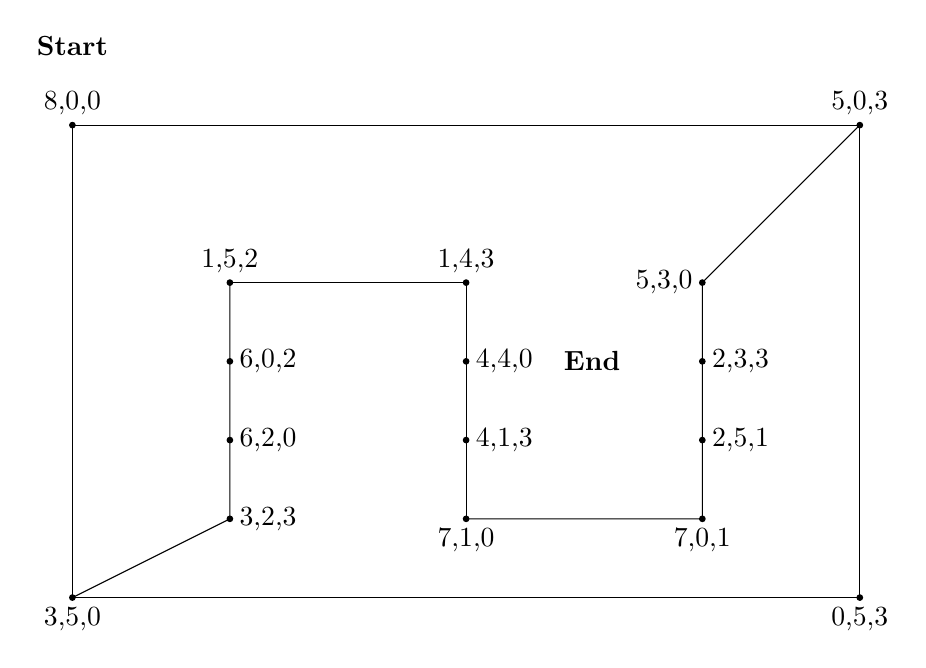
\begin{tikzpicture}
            \filldraw (0,0) circle (1pt) node[below] {3,5,0};
            \filldraw (0,6) circle (1pt) node[above] {8,0,0};
            \filldraw (10,0) circle (1pt) node[below] {0,5,3};
            \filldraw (10,6) circle (1pt) node[above] {5,0,3};

            \filldraw (2,1) circle (1pt) node[right] {3,2,3};
            \filldraw (2,2) circle (1pt) node[right] {6,2,0};
            \filldraw (2,3) circle (1pt) node[right] {6,0,2};
            \filldraw (2,4) circle (1pt) node[above] {1,5,2};

            \filldraw (5,1) circle (1pt) node[below] {7,1,0};
            \filldraw (5,2) circle (1pt) node[right] {4,1,3};
            \filldraw (5,3) circle (1pt) node[right] {4,4,0};
            \filldraw (5,4) circle (1pt) node[above] {1,4,3};

            \filldraw (8,1) circle (1pt) node[below] {7,0,1};
            \filldraw (8,2) circle (1pt) node[right] {2,5,1};
            \filldraw (8,3) circle (1pt) node[right] {2,3,3};
            \filldraw (8,4) circle (1pt) node[left] {5,3,0};

            \draw (0,0) -- (0,6) -- (10,6) -- (10,0) -- (0,0);
            \draw (0,0) -- (2,1) -- (2,2) -- (2,3) -- (2,4);
            \draw (2,4) -- (5,4) -- (5,3) -- (5,2) -- (5,1);
            \draw (5,1) -- (8,1) -- (8,2) -- (8,3) -- (8,4) -- (10,6);

            \node at (0,7) {\textbf{Start}};
            \node at (6.6,3) {\textbf{End}};
        \end{tikzpicture}
    \end{center}


    \begin{itemize}
        \item[a.]   Path:
            \solution{
                8,0,0 - 3,5,0 - 3,2,3 - 6,2,0 - 6,0,2 - 1,5,2 - 1,4,3 - 4,4,0

                There is another solution as well.
            }{ \vspace{1cm} }

        \item[b.]   What does the 1st position in the vertex label represent?
            \solution{
                The amount of water in the pail
            }{ \vspace{1cm} }

        \item[b.]   What does the 2nd position in the vertex label represent?
            \solution{
                The amount of water in jar 1
            }{ \vspace{1cm} }

        \item[c.]   What does the 3rd position in the vertex label represent?
            \solution{
                The amount of water in jar 2
            }{ \vspace{1cm} }
    \end{itemize}

\end{question}



\end{document}
